\documentclass[a4paper,12pt]{report} % добавить leqno в [] для нумерации слева

%%% Работа с русским языком
\usepackage{cmap}					% поиск в PDF
\usepackage{mathtext} 				% русские буквы в формулах
\usepackage[T2A]{fontenc}			% кодировка
\usepackage[utf8]{inputenc}			% кодировка исходного текста
\usepackage[english,russian]{babel}	% локализация и переносы

\usepackage{graphicx}				%вставка изображений(графиков, в частности)
\usepackage{listings}
\usepackage{color}

\definecolor{dkgreen}{rgb}{0,0.6,0}
\definecolor{gray}{rgb}{0.5,0.5,0.5}
\definecolor{mauve}{rgb}{0.58,0,0.82}

\lstset{frame=tb,
  language=Python,
  aboveskip=3mm,
  belowskip=3mm,
  showstringspaces=false,
  columns=flexible,
  basicstyle={\small\ttfamily},
  numbers=none,
  numberstyle=\tiny\color{gray},
  keywordstyle=\color{blue},
  commentstyle=\color{dkgreen},
  stringstyle=\color{mauve},
  breaklines=true,
  breakatwhitespace=true,
  tabsize=4
}

%%% Дополнительная работа с математикой
\usepackage{amsmath,amsfonts,amssymb,amsthm,mathtools} % AMS
\usepackage{icomma} % "Умная" запятая: $0,2$ --- число, $0, 2$ --- перечисление

%% Номера формул
\mathtoolsset{showonlyrefs=true} % Показывать номера только у тех формул, на которые есть \eqref{} в тексте.

%% Шрифты
\usepackage{euscript}	 % Шрифт Евклид
\usepackage{mathrsfs} % Красивый матшрифт

%% Свои команды
\DeclareMathOperator{\sgn}{\mathop{sgn}}

%\setlength\parindent{0ex}
%\setlength\parskip{0.3cm}

\renewcommand{\arraystretch}{1.8}

%%% Заголовок
\author{Волков Павел А-14-19}
\title{Отчет по Лабораторной работе №3}
\date{\today}

\begin{document}

\begin{titlepage}
	\newpage

	\begin{center}
	НАЦИОНАЛЬНЫЙ ИССЛЕДОВАТЕЛЬСКИЙ УНИВЕРСИТЕТ\\
		"МОСКОВСКИЙ ЭНЕРГЕТИЧЕСКИЙ ИНСТИТУТ"\\
	\end{center}

	\vspace{8em}	

	\begin{center}
		\Large Кафедра математического и компьютерного моделирования\\ 
	\end{center}

	\vspace{2em}

	\begin{center}
		\textsc{\textbf{ \Large Численные методы \linebreak Отчет по лабораторной работе №3 \linebreak "Решение систем линейных алгебраических уравнений прямыми методами. Теория возмущений." \linebreak Вариант 33}}
	\end{center}

	\vspace{6em}



	\newbox{\lbox}
	\savebox{\lbox}{\hbox{Амосова Ольга Алексеевна}}
	\newlength{\maxl}
	\setlength{\maxl}{\wd\lbox}
	\hfill\parbox{11cm}{
		\hspace*{5cm}\hspace*{-5cm}Студент:\hfill\hbox to\maxl{Волков Павел Евгеньевич\hfill}\\
		\hspace*{5cm}\hspace*{-5cm}Преподаватель:\hfill\hbox to\maxl{Амосова Ольга Алексеевна}\\
		\\
		\hspace*{5cm}\hspace*{-5cm}Группа:\hfill\hbox to\maxl{А-14-19}\\
	}


	\vspace{\fill}

	\begin{center}
		Москва \\2021
	\end{center}

\end{titlepage}

\section*{Задача 3.1}
\subsection*{Постановка задачи}

Реализовать решение СЛАУ с помощью $LU$-разложения и $LU$-разложения по схеме частичного выбора.
Решить систему небольшой размерности с возмущенной матрицей обоими методами, оценить погрешность и сравнить с теоретической оценкой. Проанализировать поведение метода с ростом числа уравнений.

$(33 + 3) mod 2 = 0$ - решение с помощью $LU$-разложения  реализовано в виде 2-х функций, одна из которых возвращает две матрицы - $L$ и $U$, не модифицируя $A$, а вторая функция решает систему, решение с помощью $LU$ по схеме частичного выбора модифицирует исходную матрицу $A$.

\[
	(33+3) mod 4 = 0 \to A_{i, j} = \tg^{17-j}(i + 1)
\]
\subsection*{Решение}
Приведем код простого LU-разложения:

\begin{lstlisting}
def LU_dec(A: np.ndarray) -> tuple:
    L = np.empty(A.shape)
    U = np.empty(A.shape)
    n = A.shape[0]
    for i in range(n):
        for j in range(n):
            U[i, j] = A[i, j]
            L[i, j] = int(i == j)
    for i in range(n):
        for j in range(i+1, n):
            L[j, i] = U[j, i] / U[i, i]
            U[j] = U[j] - L[j, i] * U[i]
    return (L, U)
\end{lstlisting}
\newpage
Метод LU-разложения по схеме частичного выбора:

\begin{lstlisting}
def swap(A: np.ndarray, L: np.ndarray, permutations: list, i: int):
    mx, line = np.abs(A[i, i]), i
    for j in range(i+1, A.shape[0]):
        if np.abs(A[j, i]) > mx:
            mx = np.abs(A[j, i])
            line = j
    for j in range(A.shape[0]):
        A[line, j], A[i, j] = A[i, j], A[line, j]
        L[line, j], L[i, j] = L[i, j], L[line, j]
    permutations[i], permutations[line] = permutations[line], permutations[i]

def LU_part(A: np.ndarray) -> tuple:
    L = np.empty(A.shape)
    n = A.shape[0]
    permutations = list(range(n))
    for i in range(n):
        for j in range(n):
            L[i, j] = int(i == j)
    for i in range(n):
        swap(A, L, permutations, i)
        for j in range(i+1, n):
            L[j, i] = A[j, i] / A[i, i]
            A[j] = A[j] - L[j, i] * A[i]
    return L, permutations
\end{lstlisting}

Точное решение системы 5 на 5 $Ax = b$, где $b = A(N, N, N, N, N)^T$:
\[
	x = (33., 33., 33., 33. , 33.)^T
\]
Теперь прибавим 0.001 к первому элементу матрицы, и найдем решения с помощью обоих методов:
\begin{gather*}
	x1 = (32.99999171, 32.99996228, 32.99998698, 33.00006978, 33.00001011)^T \\
	x2 = (32.99999171, 32.99996228, 32.99998698, 33.00006978, 33.00001011)^T
\end{gather*}

Вычислим относительную погрешность решения, и сравним ее с теоретической оценкой:
\begin{gather*}
	\delta(x^*) = \dfrac{|| \bar{x} - x^*||}{||x^*||} = 1.143\cdot 10^{-6} \\
	\delta(b^*) = 0 \\
	\delta(A^*) = \dfrac{|| A - A^*||}{||A||} = 7.177 \cdot 10^{-13}\\
	\nu_{\delta} = cond(A) = ||A|| \cdot ||A^{-1}|| = 1.265 \cdot 10^{20}\\
\end{gather*}

Таким образом, неравенство $\delta(x^*) \leq \nu_{\delta} \cdot (\delta(b^*) + \delta(A^*)) = 1.143\cdot 10^{-6} \leq 90.805552 \cdot 10^6$ выполняется.

Ниже представлен графики зависимости относительной погрешности решения от числа уравнений для обоих методов:

\noindent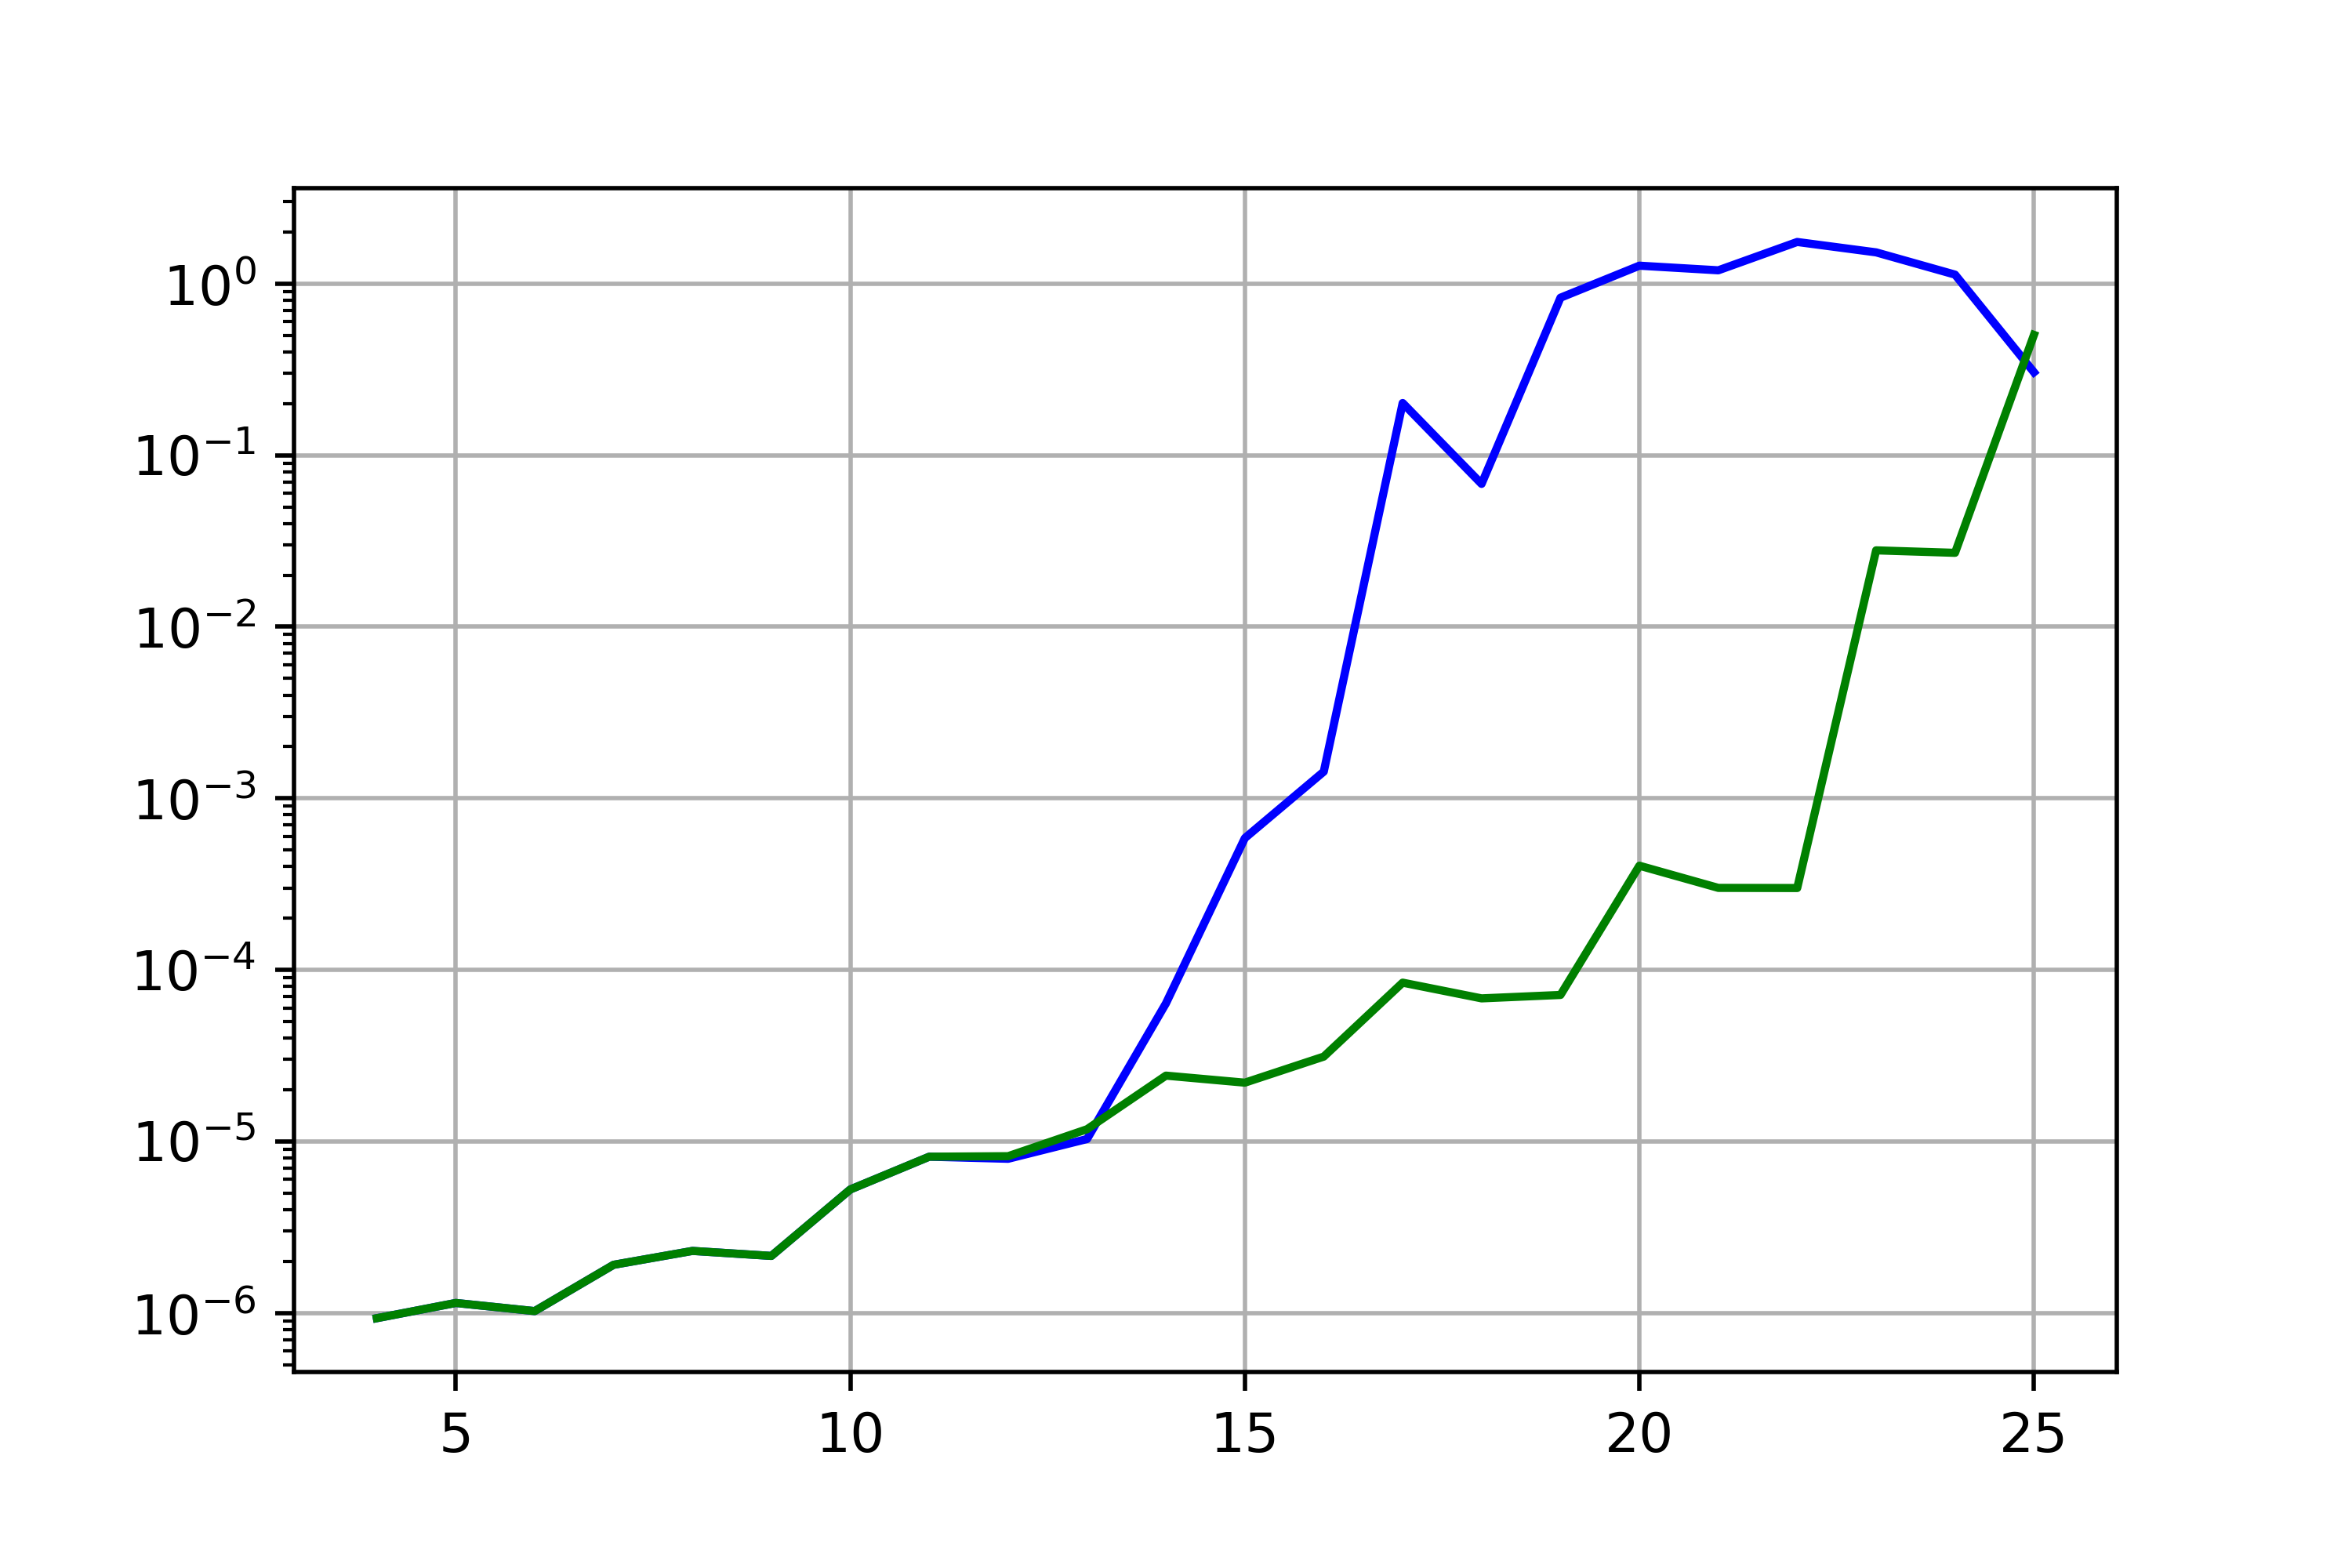
\includegraphics{3.1_plot.png}

На графике видно, что благодаря перестановкам строк, и выбору ведущими элементами наибольших по модулю в столбце,
метод частичного выбора сохраняет относительную погрешность менее 1\% для числа уравнений < 23, а метод без перестановок < 17.

\section*{Задача 3.2}
\subsection*{Постановка задачи}

Дана система уравнений $Ax = b$ порядка $n$ с разреженной матрицей $A$. Решить систему прямым методом.

В случае коллизий в матрице, диагонали имеют приоритет над столбцами, главные диагонали - над побочными.

$n = 65$ На главной диагонали элементы равны 87, на 23-й наддиагонали элементы равны 30, на 2-й побочной поддиагонали элементы равны 4. ($b_i = n \cdot i + n$) 
\subsection*{Решение}

\section*{Задача 3.3}
\subsection*{Постановка задачи}

Решить задачу итерационным методом, указанным в индивидуальном варианте. Вектор правой части задается как $b = Ax$, где $x_i = 33$

Элементы матрицы $A$ задаются формулами \newline $a_{i, j} = \dfrac{\cos{i + j}}{0.1 \cdot \beta} + 0.1\beta \cdot e^{-(i - j)^2}$.

Параметр $\beta$ задается формулой $\beta = (|66 - 33| + 5) \cdot m$, здесь N - номер варианта, m - размерность матрицы, указанная в варианте. Вектор b задается по вектору решения.

m = 26, метод минимальных невязок.


\subsection*{Решение}

\end{document}